\section{Question 1}
\begin{figure}[!ht]
	\centering
	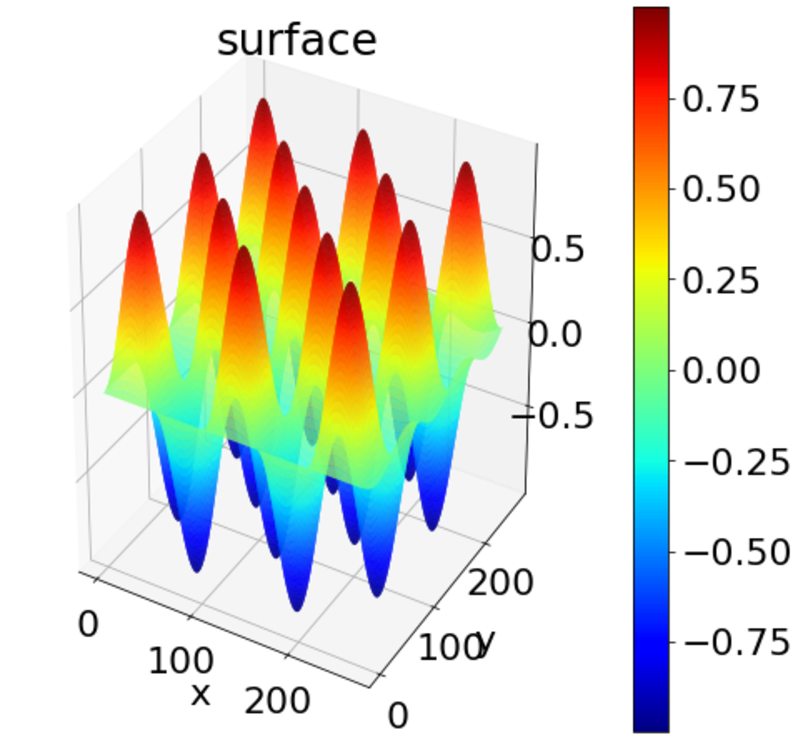
\includegraphics[scale=0.5]{surf_0.pdf}
	\caption{Surface plot of global solution, order 8, at time 0}
\end{figure}

\begin{figure}[!ht]
	\centering
	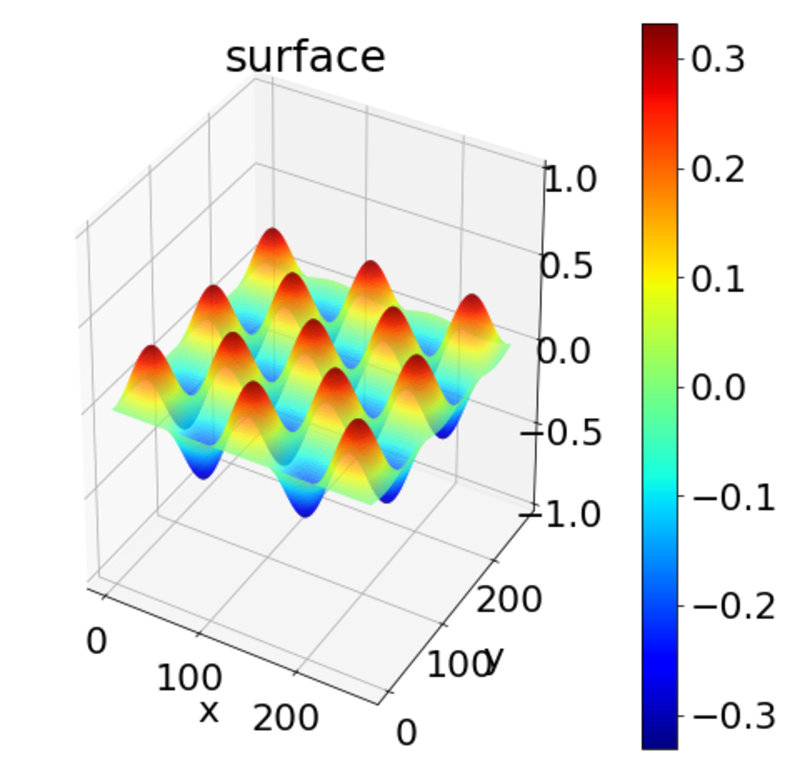
\includegraphics[scale=0.5]{surf_1.pdf}
	\caption{Surface plot of global solution, order 8, at time 1000}
\end{figure}

\begin{figure}[!ht]
	\centering
	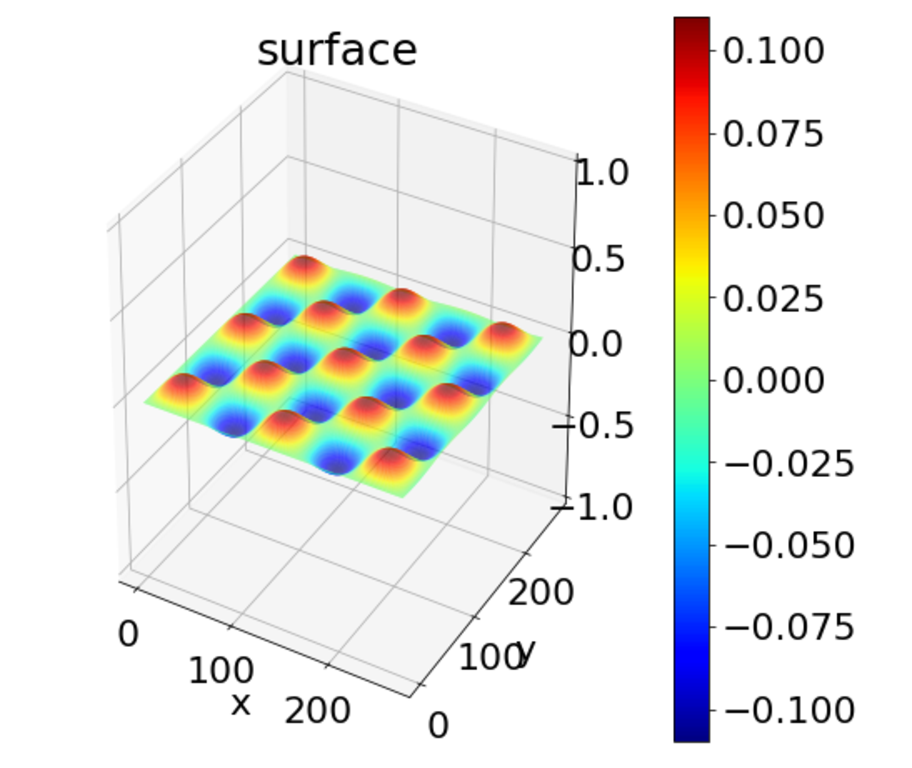
\includegraphics[scale=0.5]{surf_2.pdf}
	\caption{Surface plot of global solution, order 8, at time 2000}
\end{figure}


\section{Question 2}
See code

\section{Question 3}
The algorithms were all run for 400 timesteps. For the block algorithm we used 8 steps per thread in the y direction and 8 threads per block in the y direction. In total we used 256 threads per block.
\begin{figure}[!ht]
	\centering
	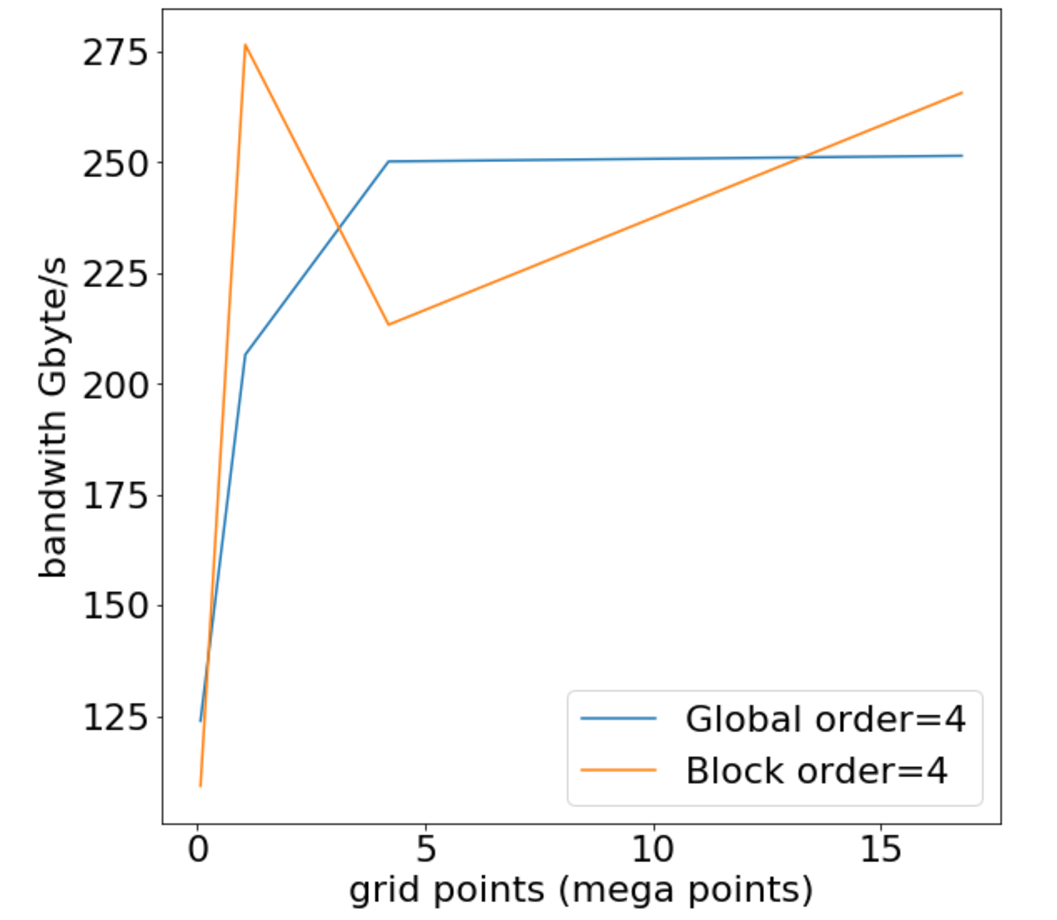
\includegraphics[scale=0.5]{graph_alg.pdf}
	\caption{Comparison of bandwidth for Global and Block algorithm of order 4}
\end{figure}

\begin{figure}[!ht]
	\centering
	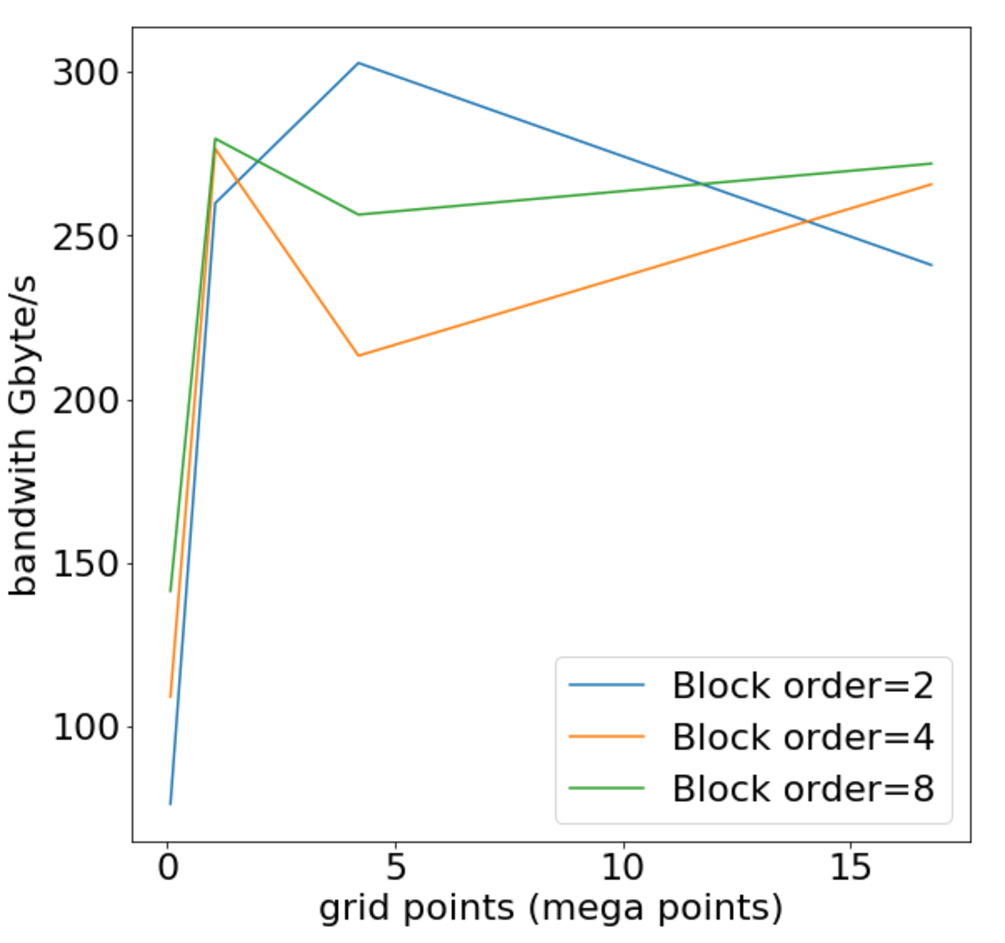
\includegraphics[scale=0.5]{graph_block.pdf}
	\caption{Comparison of bandwidth for Block algorithm of varying order}
\end{figure}

\section{Question 4}


